\documentclass[tikz, border=2pt]{standalone}

\usepackage{amsmath,amssymb}
\usepackage{pgfplots}
\pgfplotsset{compat=1.18}
\usepgfplotslibrary{groupplots}
\usetikzlibrary{arrows.meta}
\usepackage{xcolor}

\definecolor{utnblue}{RGB}{0, 51, 102}

\begin{document}
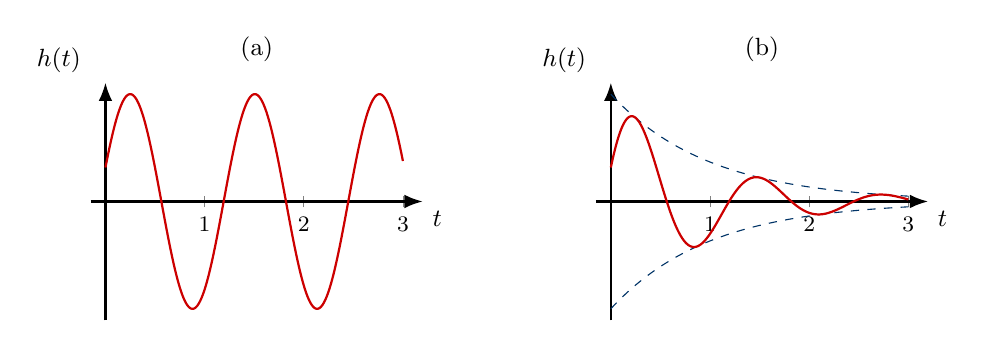
\begin{tikzpicture}[>=Latex, font=\small]

\pgfplotsset{
  every axis/.append style={
    axis lines=middle,
    axis line style={->, thick, black},
    width=5.8cm, height=4.6cm,
    xlabel={$t$}, ylabel={$h(t)$},
    xlabel style={anchor=north west},
    ylabel style={rotate=0, anchor=south east, at={(axis description cs:0,1)}},
    xmin=-0.15, xmax=3.2,
    ymin=-7, ymax=7,
    ytick=\empty,
    xticklabel style={font=\footnotesize},
    title style={yshift=-2pt},
    samples=300,
    clip=false,
  },
  resp/.style={red!80!black, thick},
  env/.style={utnblue, thin, dashed},
}

\begin{groupplot}[
  group style={group size=2 by 1, horizontal sep=2.2cm},
]
  % ===== (a) sostenida: 2[cos 5t + 3 sin 5t] =====
  \nextgroupplot[domain=0:3, title={(a)}]
    \addplot[resp] {2*cos(deg(5*x)) + 6*sin(deg(5*x))};

  % ===== (b) amortiguada: 2 e^{-t}[cos 5t + 3 sin 5t] =====
  \nextgroupplot[domain=0:3, title={(b)}]
    \addplot[env] {6.32*exp(-x)};
    \addplot[env] {-6.32*exp(-x)};
    \addplot[resp] {exp(-x)*(2*cos(deg(5*x)) + 6*sin(deg(5*x)))};
\end{groupplot}
\end{tikzpicture}
\end{document}
